\documentclass{beamer}

\usepackage[noline, noend]{algorithm2e} % algorithmn
\usepackage{amsmath}
\usepackage{amsbsy}
\usepackage{bbm}
\usepackage[utf8]{inputenc}
\usepackage{hyperref}
\hypersetup{
    colorlinks=true,
    linkcolor=blue,
    filecolor=magenta,      
    urlcolor=cyan,
}


\usepackage{utopia} %font utopia imported
\usepackage{lmodern}

\graphicspath{{./images/}} 


\newcommand{\matr}[1]{\mathbf{#1}}
\newcommand{\norm}[1]{\left\lVert#1\right\rVert}
\newcommand{\E}[2][]{\mathbb{E}_{#1}\left\{#2\right\}}
\newcommand{\var}[2][]{var_{#1}\left\{#2\right\}}
\newcommand{\cov}[1]{cov\{#1\}} 
\newcommand{\normal}[1]{\mathcal{N}\left(#1\right)}
\newcommand{\exponents}[1]{exp\left\{#1\right\}}
\newcommand{\indicator}[1]{\mathbbm{1}_{#1}}

\newcommand{\bmu}{\boldsymbol{\mu}}
\newcommand{\bpi}{\boldsymbol{\pi}}
\newcommand{\bTheta}{\boldsymbol{\Theta}}
\newcommand{\bSigma}{\boldsymbol{\Sigma}}
\newcommand{\bphi}{\boldsymbol{\phi}}

\newcommand{\calA}{\mathcal{A}}
\newcommand{\calL}{\mathcal{L}} 
\newcommand{\calE}{\mathcal{E}}
\newcommand{\calR}{\mathcal{R}}
\newcommand{\calC}{\mathcal{C}}
\newcommand{\calD}{\mathcal{D}}
\newcommand{\bx}{\matr{x}}
\newcommand{\bt}{\matr{t}}
\newcommand{\bw}{\matr{w}}
\newcommand{\bX}{\matr{X}}
\newcommand{\bZ}{\matr{Z}} 
\newcommand{\bz}{\matr{z}}
\newcommand{\bu}{\matr{u}}
\newcommand{\bY}{\matr{Y}}

\usetheme{Madrid}
\usecolortheme{default}

\title[]{Monte Carlo Simulation on Credit Risk}
\author[Loora, Peiqi]{Loora Li \and Peiqi Wang \and Zeneng Fan \and Xiaoye Yuan \and Jiayi Zhang}
\date[July 5th, 2018]{Supervisor: Prof. Ken Jackson }


\begin{document}

\frame{\titlepage}
\begin{frame}
    \frametitle{Overview}
    \tableofcontents
\end{frame}


%---------------------------------------------------------
\section{Monte Carlo Simulation}
%---------------------------------------------------------


\begin{frame}
\frametitle{MC is about Sampling and Averaging!}
\begin{enumerate} 
    \item To simulate some unknown value $\mu$, we interpret $\mu$ probabilistically, i.e. expresses it as the expected value of a function of some random variable $X$
    \[
        \mu = \E[\bX \sim p(\bX)]{f(\bX)}
    \]
    \item Sample $X_1, \cdots, X_n \overset{i.i.d.}{\sim} p$ , and compute the Monte Carlo (MC) estimator
    \[
        \hat{\mu} = \frac{1}{n} \sum_{i=1}^n f(\bX_i)
    \]
\end{enumerate}    
\begin{center}
    
\includegraphics{slight.png}
\end{center}
\end{frame}

\begin{frame}{Gif Demo} 
\begin{center}
    
\includegraphics[width=0.5\textwidth]{link_shaking.png} \\ 
    \href{https://en.wikipedia.org/wiki/Monte_Carlo_method}{link} \\    
\end{center}
\end{frame}



% explain LLN:
%     for any nonzero margin specified, no matter how small, with a sufficiently large sample there will be a very high probability that the average of the observations will be close to the expected value; that is, within the margin.


\begin{frame}{How to get a better MC estimator?}
We evaluate an estimator by computing
\begin{align*}
    \E{\hat{\mu}} &= \frac{1}{n} \sum_{i=1}^n \E{f(\bX_i)} = \mu \quad \text{(Accuracy)} \\ 
     \var{\hat{\mu}} &= \frac{1}{n^2}\sum_{i=1}^n \var{f(\bX_i)} = \frac{\sigma^2}{n} \quad \text{(Precision)}
\end{align*}
where $\E{\bX_i} = \mu$ and $\var{\bX_i}=\sigma^2$. 
\begin{center}
    
\includegraphics{shy.png}
\end{center}
\end{frame}


% Intuitively, estimator is more precise, i.e. smaller CI, with decreased variance. 
% talk about how sample size and variance affect performance of an estimator
% motivate reducing estimator's variance by somehow reducing the random variable's variance


\begin{frame}{Variance Reduction trick: importance sampling!}
\textbf{Motivation} In the case of estimating rare events, we want to compute $\mu = \E{f(\bX)}$ where $f(\bX)$ is close to zero out side of a region $\mathcal{D}$. 
% We can exploit this to do variance reduction with \textbf{importance sampling}
\begin{enumerate}
    \item Consider any \textit{proposal distributions} $q(\bX)$ to sample from instead of $p(\bX)$, i.e. $X_1, \cdots, X_n \sim q(\bX)$. 
    % (If $q(\bX)$ in exponential family, then IS procedure is called \textit{exponential twisting})
    \item Adjust the estimates such that the MC estimates \textbf{remains unbiased}
    \begin{align*}
        \mu = \E[\bX \sim p]{f(\bX)} 
        &= \int_{\mathcal{D}} f(\bx) p(\bx) d\bx \\
        &= \int_{\mathcal{D}} \frac{f(\bx)p(\bx)}{q(\bx)} q(\bx) d\bx 
        = \E[\bX \sim q]{\frac{f(\bX)p(\bX)}{q(\bX)}}
    \end{align*}
    where $\frac{p(\bX)}{q(\bX)}$ is the \textit{likelihood} $L(\bX)$, i.e. the adjustment
    \item Optimize for $q(\bX)$ such that \textbf{variance is reduced/minimized}
    \[
        \var[\bX \sim q]{f(\bX) L(\bX)} < 
        \var[\bX \sim p]{f(\bX)}
    \]
\end{enumerate}
\begin{center}
    
\includegraphics{surprise.png}
\end{center}
\end{frame}

% mention require using optimization techniques ...
% how well the IS performs depends heavily on finding the right q(X), a bad parameter will result in larger variance, i.e. worst performance. But when done right, huge time saving!

%---------------------------------------------------------
\section{Problem Setup}
%---------------------------------------------------------
 
\begin{frame}{Need to know some basic finance :)}
\begin{enumerate}
    \item \textbf{Portfolio} A collection of investments / loans
    \item \textbf{Credit Risk} Risk of default in a portfolio
    \item \textbf{Systemic Risk} Overall risk that affects all assets, i.e. government policy, international economic forces, or acts of nature.
    \item \textbf{Idiosyncratic Risk} Risk endemic to a particular asset, i.e. aspects of a company
\end{enumerate}
\begin{center}
    
\includegraphics{shrunken.png}
\end{center}
\end{frame}



\begin{frame}{A Credit Risk Model}
\textbf{Guassian Copula Factor Model} 
% is a model that measure credit risk by modeling a set of underlying risk factors as Gaussian random variables. 
\begin{enumerate}
    \item Given probability of default for $k$th borrower, $p_k$ (i.e. $p_k = 0.01$)
    \item Let $Y_k$ be the default indicator for the $k$th borrower.
    \[
        Y_k = \mathbbm{1}_{X_k > x_k} \qquad \text{$x_k$ picked to match $p_k$, i.e. } \E{Y_k} = p_k
    \]
    where $X_k$ is a weighted sum of the risk factors
    \[
        X_k = \boldsymbol{\beta}_k^T \matr{Z}  + \sqrt{1 - \boldsymbol{\beta}_k^T \boldsymbol{\beta}_k} \epsilon_k
    \]
    given systematic risk factors $Z \sim \normal{0,I_S}$ and idiosyncratic risk factors $\epsilon \sim \normal{0,I_N}$
%  i.e. 1 if $k$th borrower defaults with probability $p_k$ and 0 otherwise with probability of $1-p_k$.
    \item $L$ is the total loss from defaults
    \[
        L = c_1 Y_1 + \cdots + c_N Y_N    
    \]
% where $c_k$ is the loss resulting from default of $k$th borrower 
\end{enumerate}
\begin{center}
    
\includegraphics{wave.png}
\end{center}
\end{frame}



\begin{frame}{MC and 2 Level IS applied to the Copula Model}
We are interested in the \textit{probability that a given portfolio of lenders will result in a loss greater than a specified amount}. And we use \textit{Monte Carlo simulation} to estimate this probability
\begin{align*}
    P(L \geq l) 
    &= \E[\bZ \sim \normal{0, I_S}\,\, Y_k \sim p_k]{\mathbbm{1}_{L \geq l}}
\end{align*}
We can apply \textit{importance sampling} for variance reduction when estimating this probabilistically
\begin{center}
    
\includegraphics{trick.png}
\end{center}
% . Because there are two underlying factors in the copula factor model, i.e. systematic $\bZ$ and idiosyncratic $\epsilon_k$ or equivalently $Y_k$, we perform \textbf{importance sampling twice}. \\
% $ $\\
% \textit{Motivation}: Applying IS to outer level (i.e. sampling $\bZ$) improves performance for strongly correlated borrowers and applying IS in inner level (i.e. sampling $Y_k$) improves performance for weakly correlated borrowers
\end{frame}

\begin{frame}{The Algorithm with Two level IS!}
\begin{center}
\begin{algorithm}[H]
    Find $\mu$, parameter for optimal $\bZ$ proposal distribution \\
    Sample $\{Z_i\}_{i=1}^{NZ} \sim \normal{\mu, I_S}$ \\
    \For{$1$ \KwTo $NZ$}{
        Find $p_{k,\theta}$, parameter for optimal $Y_k$ proposal distribution \\
        Sample $\{ Y_k^i \}_{i=1, k=1}^{NZ, NE} \sim p_{k,\theta}$ \\
        \For{$1$ \KwTo $NE$}{
            $\mathcal{L}_{ij} \leftarrow c_1 Y_1^i + \cdots + c_n Y_N^i$ \\
            $a_{ij} \leftarrow \mathbbm{1}_{\{L_{ij} > l\}} e^{-\theta \mathcal{L}_{ij} + \psi} e^{-\mu^T \bZ + \mu^T \mu / 2}$ \\
        }
    }
    \Return{$mean(a_{ij})$}
\end{algorithm}
\end{center}
\begin{center}
    
\includegraphics{speechless.png}
\end{center}
\end{frame}

\section{Question to be answered}

\begin{frame}{Problem: Two level IS MC estimator is biased downward}
\begin{center}
    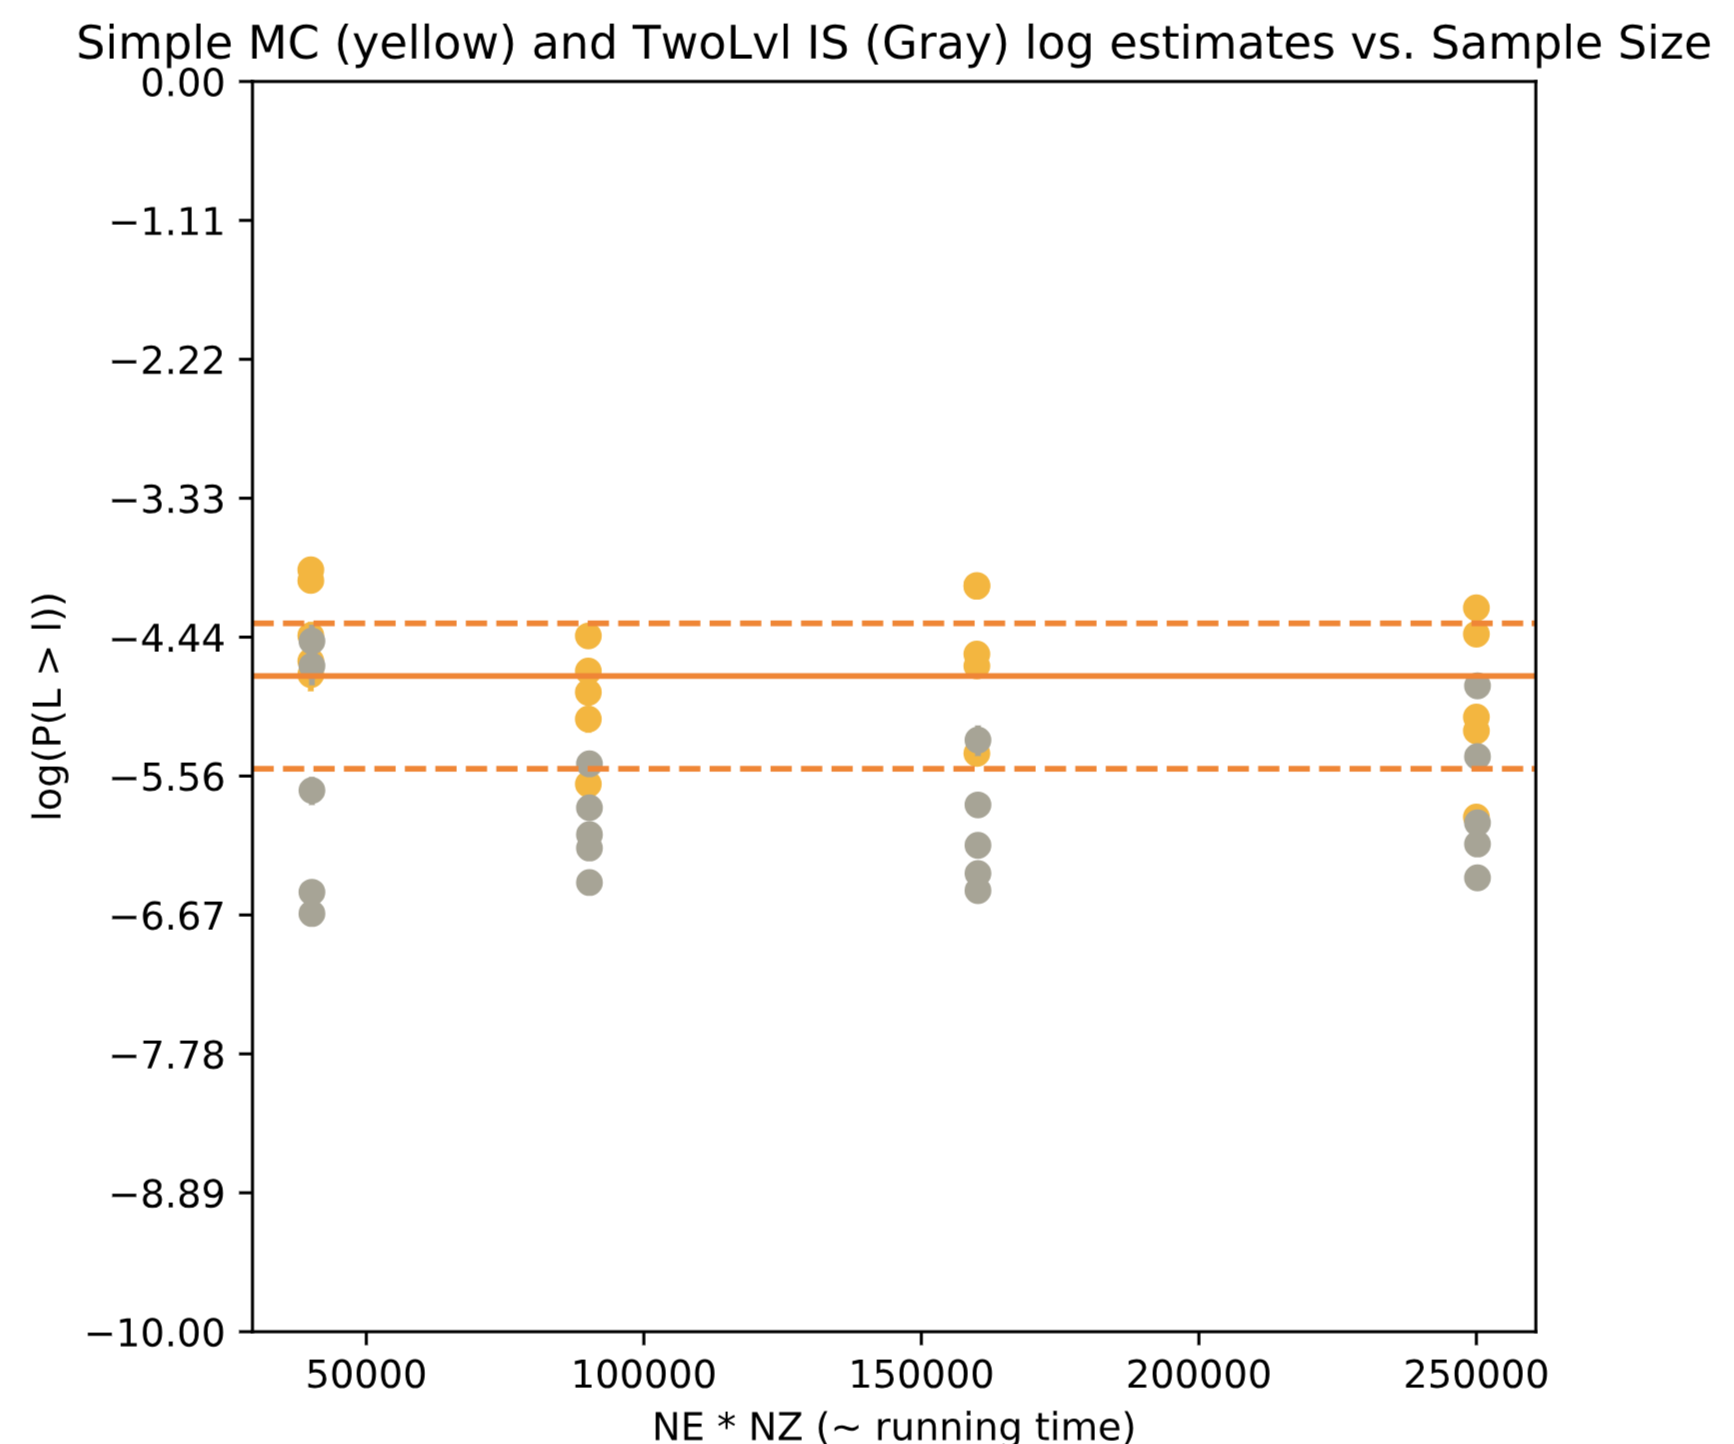
\includegraphics[width=0.70\textwidth]{gl_downward_bias.png}
\end{center}
observed from Adam Sturge's master thesis.
\end{frame}

\begin{frame}{Next Steps}
\begin{center}
    \begin{enumerate}
        \item \textbf{Increase Sample Size}
        \item \textbf{Look into Outer Lever IS: the Selection of $\mu$}
    \end{enumerate}
\end{center}
\end{frame}

\begin{frame}
\begin{center}
    \textbf{\textit{Thanks!}} \\
    $ $\\
    
\includegraphics[width=\textwidth]{botw_view.jpg}
\end{center}
\end{frame}


\end{document}   